\section{Evaluadores}
Los evaluadores permiten especificar puntos en una curva o superficie simplemente usando puntos de control. La curva o la superficie se pueden mostrar con cualquier precisión.\\

Una curva de Bézier es una función vectorial de una variable.

\begin{align*}
C\left(u\right)=[X\left(u\right)Y\left(u\right)Z\left(u\right)]
\end{align*}
Donde $u$ varía en un dominio $[0,1]$. \\

Una superficie de Bézier es una función vectorial de dos variables.

\begin{align*}
S\left(u,v\right)=[X\left(u,v\right)Y\left(u,v\right)Z\left(u,v\right)]
\end{align*}
Donde $u$ y $v$ pueden variar en algún dominio. El rango no es necesariamente tridimensional como se muestra. Puede tener una salida bidimensional para curvas en un plano o coordenadas de textura, o una salida cuatridimensional para especificar información RGBA. Incluso la salida unidimensional puede tener sentido para los niveles de gris.\\

Para cada u (u y v, en el caso de una superficie), la fórmula de  \textbf{C()} o \textbf{S()} calcula un punto de la curva o superficie. Para utilizar un evaluador, primero hay que definir la función \textbf{C()} o \textbf{S()}, habilitarla y luego utilizar el comando \textbf{glEvalCoord1()} o \textbf{glEvalCoord2()} en lugar de \textbf{glVertex*()}. De este modo, los vértices de la curva o de la superficie pueden utilizarse como cualquier otro vértice, para formar puntos o líneas. Además, otros comandos generan automáticamente series de vértices que producen una malla regular uniformemente espaciada en u (o en u y v). Los evaluadores unidimensionales y bidimensionales son similares, pero la descripción es algo más sencilla en una dimensión.
%%%%%%%%%%%%%%%%%%%%%%%%%%%%%%%%%%%%%%%%%%%%%%%%%%%%%%%%%%%%%%%%%%%%%%%%%%%%%
\subsection{Evaluadores unidimensionales}
Presentamos un ejemplo del uso de evaluadores unidimensionales para dibujar una curva. A continuación, se describen los comandos y ecuaciones que controlan los evaluadores.\\

\textbf{Ejemplo unidimensional:} Una curva de Bézier simple.\\

El programa mostrado en el Ejemplo 1 dibuja una curva cúbica de Bézier usando cuatro puntos de control, como se muestra en la Figura 1.

\begin{figure}[h!]
	\centering
	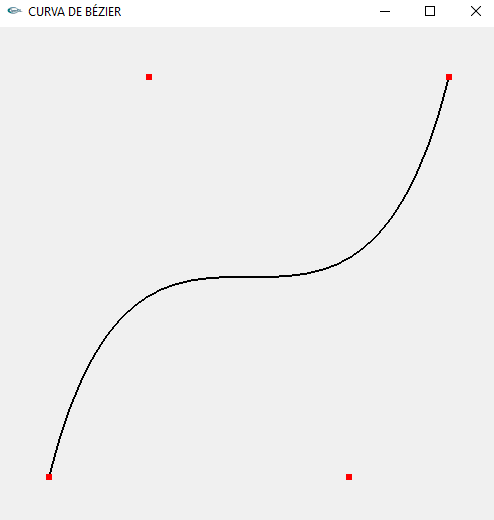
\includegraphics[width=0.5\linewidth]{../images/CURVA.PNG}
	\caption{Curva de Bézier.}
	\label{fig:propuesta}
\end{figure}
%%%%%%%%%%%%%%%%%%%%%%%%%%%%%%%%%%%%%%%%%%%%%%%%%%%%%%%%%%%%%%%%%%%%%%%%%%%%%%%%%%%%%%%%%%%%%%%%%%%%%%%%%%%%%%%%%%%%%%%%%%%%%%%%%%%%%%%%%%%%%%%%%%%%%%%%%%%%%%%%%%%%%%%%%%%%%%%%%%%%%%%%%%%%%%%%%%%%%%%%%%%%%%%%%%%%%%%%%%%%%%%%%%%%%%%%%%%%%%%%%%%%%%
\subsubsection{Código del ejemplo}

\lstset{language=C, breaklines=true, basicstyle=\footnotesize}
\begin{lstlisting}
#include <windows.h>
#include <GL/gl.h>
#include <GL/glu.h>
#include <stdlib.h>
#include <GL/glut.h>

GLfloat ctrlpoints[4][3] = {{ -4.0, -4.0, 0.0}, { -2.0, 4.0, 0.0},
                            {2.0, -4.0, 0.0}, {4.0, 4.0, 0.0}};

void init(void){
  glClearColor(0.0, 0.0, 0.0, 0.0);
  glShadeModel(GL_FLAT);
  glMap1f(GL_MAP1_VERTEX_3, 0.0, 1.0, 3, 4, &ctrlpoints[0][0]);
  glEnable(GL_MAP1_VERTEX_3);
}

void display(void){
      int i;
      glClear(GL_COLOR_BUFFER_BIT);
      glColor3f(1.0, 1.0, 1.0);

      glBegin(GL_LINE_STRIP);
        for (i = 0; i <= 30; i++)
            glEvalCoord1f((GLfloat) i/30.0);
      glEnd();

 /* El siguiente codigo muestra los puntos de control como puntos. */
      glPointSize(5.0);
      glColor3f(1.0, 1.0, 0.0);
      glBegin(GL_POINTS);
        for (i = 0; i < 4; i++)
          glVertex3fv(&ctrlpoints[i][0]);
      glEnd();

glFlush();
}

void reshape(int w, int h) {
      glViewport(0, 0, (GLsizei) w, (GLsizei) h);
      glMatrixMode(GL_PROJECTION);
      glLoadIdentity();

      if (w <= h)
        glOrtho(-5.0, 5.0, -5.0*(GLfloat)h/(GLfloat)w,
        5.0*(GLfloat)h/(GLfloat)w, -5.0, 5.0);
      else
      glOrtho(-5.0*(GLfloat)w/(GLfloat)h,
      5.0*(GLfloat)w/(GLfloat)h, -5.0, 5.0, -5.0, 5.0);
      glMatrixMode(GL_MODELVIEW);
      glLoadIdentity();
}

int main(int argc, char** argv) {
      glutInit(&argc, argv);
      glutInitDisplayMode (GLUT_SINGLE | GLUT_RGB);
      glutInitWindowSize (500, 500);
      glutInitWindowPosition (100, 100);
      glutCreateWindow (argv[0]);
      init ();
      glutDisplayFunc(display);
      glutReshapeFunc(reshape);
      glutMainLoop();
      return 0;
}
\end{lstlisting}

La curva cúbica de Bézier se describe mediante cuatro puntos de control, que aparecen en este ejemplo en la matriz \textbf{ctrlpoints[][]}. Esta matriz es uno de los argumentos de \textbf{glMap1f()}. Todos los argumentos de este comando son los siguientes:\\
\begin{itemize}
    \item \textbf{$GL\_MAP1\_VERTEX\_3$ :} Proporciona puntos de control tridimensionales y se producen vértices tridimensionales.
    \item \textbf{0.0: } Valor bajo del parámetro u
    \item \textbf{1.0: } Valor elevado del parámetro u
    \item \textbf{3: } El número de valores de punto flotante para avanzar en los datos entre un punto de control y el siguiente.
    \item \textbf{4: } El orden de la spline, que es el grado + 1: en este caso, el grado es 3 (ya que se trata de una curva cúbica ).
    \item \textbf{\&ctrlpoints[0][0]: } Puntero a los datos del primer punto de control
\end{itemize}
Nótese que el segundo y tercer argumento controlan la parametrización de la curva ya que la variable $u$ va de 0 a 1, la curva va de un extremo a otro. La llamada a \textbf{glEnable()} habilita el evaluador unidimensional para vértices tridimensionales. \\

La curva se dibuja en la rutina \textbf{display()} entre las llamadas \textbf{glBegin()} y \textbf{glEnd()}. Como el evaluador está habilitado, el comando \textbf{glEvalCoord1f()} es como emitir un comando \textbf{glVertex()} con las coordenadas de un vértice de la curva correspondiente al parámetro de entrada $u$.

%%%%%%%%%%%%%%%%%%%%%%%%%%%%%%%%%%%%%%%%%%%%%%%%%%%%%%%%%%%%%%%%%%%%%%%%%%%%%%%%%%%%%%%%%
\subsection{Definición y evaluación de un evaluador unidimensional}
El polinomio de Bernstein de grado n (u orden $n+1$ ) aproxima una función en un intervalo y viene dado por:

\begin{align*}
B_i^n\left(u\right)=\left(\begin{matrix}n\\i\\\end{matrix}\right)u^i\left(1-u\right)^{n-i}
\end{align*}
Si $Pi$ representa un conjunto de puntos de control (unidimensionales, bidimensionales, tridimensionales o incluso cuatridimensionales), entonces la ecuación:
\begin{align*}
C\left(u\right)=\sum_{i=0}^{n}{B_i^n\left(u\right)}P_i
\end{align*}
Donde los ${\displaystyle B_{i}^{n}(u)}$ son elementos de la distribución binomial respecto de la variable $u$ y los $P_{i}$ son valores de la función que queremos aproximar.\\

Representa una curva de Bézier cuando $u$ varía de 0 a 1. Para representar la misma curva, pero permitiendo que, $u$ varíe entre $u1$ y $u2$ en lugar de 0 y 1, evaluamos:
\begin{align*}
C\left(\frac{u-u_1}{u_2-u_1}\right)
\end{align*}
El comando \textbf{glMap1()} define un evaluador unidimensional que utiliza estas ecuaciones.\\

\begin{lstlisting}
    void glMap1(GLenum target,TYPE u1,TYPE u2,GLint stride,

                    GLint order,const TYPE *points);
\end{lstlisting}
El parámetro objetivo especifica lo que representan los puntos de control, como se muestra en la Tabla 1, y por lo tanto cuántos valores deben ser suministrados en puntos. Los puntos pueden representar vértices, datos de color RGBA, vectores normales o coordenadas de textura. Por ejemplo, con \textbf{$GL\_MAP1\_COLOR\_4$}, el evaluador genera datos de color a lo largo de una curva en el espacio de color de cuatro dimensiones (RGBA). También se utilizan los valores de los parámetros listados en la Tabla 1 para activar cada evaluador definido antes de invocarlo. Pase el valor apropiado a \textbf{glEnable()} o \textbf{glDisable()} para activar o desactivar el evaluador.\\

Los dos segundos parámetros de \textbf{glMap1*()}, $u1$ y $u2$, indican el rango de la variable $u$. La variable stride es el número de valores de precisión simple o doble (según el caso) en cada bloque de almacenamiento. Por lo tanto, es un valor de desplazamiento entre el comienzo de un punto de control y el comienzo del siguiente. \\

El orden es el grado más uno, y debe coincidir con el número de puntos de control. Los puntos apuntan a la primera coordenada del primer punto de control. Utilizando la estructura de datos de ejemplo para \textbf{glMap1*()}, utilice lo siguiente para los puntos:
\begin{align*}
(GLfloat \ *) (\&ctrlpoints[0].x)
\end{align*}

\begin{table}[h]
\begin{center}
\caption{Tipos de puntos de control para \textbf{glMap1*()}.}
	\arrayrulecolor{grayblack}
	%\rowcolors{1}{white}{gray}
	{\color{grayblack}
\begin{tabular}{ p{6.5cm} cc }
\toprule
\textbf{Parámetro } & \textbf{Significado} \\
\midrule
GL\_MAP1\_VERTEX\_3 & coordenadas de los vértices x, y, z.\\

GL\_MAP1\_VERTEX\_4 & coordenadas de los vértices x, y, z, w. \\
GL\_MAP1\_INDEX & índice de color. \\

GL\_MAP1\_COLOR\_4 & R, G, B, A. \\

GL\_MAP1\_NORMAL & coordenadas normales. \\

GL\_MAP1\_TEXTURE\_COORD\_1 & s coordenadas de textura. \\

GL\_MAP1\_TEXTURE\_COORD\_2 & s, t coordenadas de textura. \\

GL\_MAP1\_TEXTURE\_COORD\_3  & s, t, r coordenadas de textura \\

GL\_MAP1\_TEXTURE\_COORD\_4  & s, t, r, q coordenadas de textura. \\
\bottomrule
\end{tabular}}
\label{tab:coeficientes}
\end{center}
\end{table}

Se puede evaluar más de un evaluador a la vez. Se tiene un evaluador GL\_MAP1\_VERTEX\_3 y un evaluador GL\_MAP1\_COLOR\_4 definidos y habilitados, entonces las llamadas a \textbf{glEvalCoord1()} generan tanto una posición como un color. Sólo uno de los evaluadores de vértices puede estar habilitado a la vez, aunque se hayan definido ambos. Del mismo modo, sólo uno de los evaluadores de textura puede estar activo. Sin embargo, aparte de esto, los evaluadores pueden utilizarse para generar cualquier combinación de datos de vértices, vectores normales, colores y coordenadas de textura. Si se define y activa más de un evaluador del mismo tipo, se utiliza el de mayor dimensión. Utilizamos \textbf{glEvalCoord1*()} para evaluar un mapa unidimensional definido y habilitado.

\begin{lstlisting}
      void glEvalCoord1{fd}(TYPE u);
      void glEvalCoord1{fd} v (TYPE *u);
\end{lstlisting}
Provoca la evaluación de los mapas unidimensionales habilitados. El argumento $u$ es el valor (o un puntero al valor, en la versión vectorial del comando) de la coordenada del dominio. \\

%%%%%%%%%%%%%%%%%%%%%%%%%%%%%%%%%%%%%%%%%%%%%%%%%%%%%%%%%%%%%%%%%%%%%%%%%%%%%%%%%%%%%%%%%%%%%%%%
\subsection{Definición de valores de coordenadas uniformes en una dimensión}

Se utiliza \textbf{glEvalCoord1()} con cualquier valor para $u$, pero el uso más común es con valores espaciados uniformemente, como se muestra en el Ejemplo 1. Para obtener valores uniformemente espaciados, definimos una unidimensional usando \textbf{glMapGrid1*()} y luego aplíquelo usando \textbf{glEvalMesh1()}.

\begin{lstlisting}
    void glMapGrid1{fd} (GLint n, TYPE u1, TYPE u2);
\end{lstlisting}
Define una cuadrícula que va de $u1$ a $u2$ en $n$ pasos, que están espaciados uniformemente.
\begin{lstlisting}
    void glEvalMesh1(GLenum mode, GLint p1, GLint p2);
\end{lstlisting}

Aplicamos la cuadrícula de mapa definida actualmente a todos los evaluadores habilitados. El modo puede ser \textbf{GL\_POINT o GL\_LINE}, dependiendo de si desea dibujar puntos o una línea conectada a lo largo de la curva. La llamada tiene exactamente el mismo efecto que emitir una \textbf{glEvalCoord1()} para cada uno de los pasos, incluyendo $p1$ y $p2$, donde $0\le\ p1,\ p2\le\ n$. Es equivalente a lo siguiente: \\

\begin{lstlisting}
    glBegin(GL_POINTS); /* OR glBegin(GL_LINE_STRIP); */
          for (i = p1; i <= p2; i++)
              glEvalCoord1(u1 + i*(u2-u1)/n);
    glEnd();
\end{lstlisting}

Excepto que si $i = 0$ o $i = n$, entonces se llama a \textbf{glEvalCoord1()} con exactamente $u1$ o $u2$ como parámetro.
